%% ----------------------------------------------------------------
\chapter{Implementation}
%% ----------------------------------------------------------------


\subsection{Camera Module}
\label{sec:John_Implementation}

The first step in the implementation of the camera module was to verify the communication with the camera by talking to it via a pc. Once this step was complete the next step was to implement communications between the camera and a microprocessor, with the pc for debugging. With the microcontroller able to communicate with the camera this module was ready for integration with the payload.

\subsubsection{First camera}


\section{Communication with Ground Station via Autopilot (mh)}
\label{sec:payload controller}
Considering the overall aim of this project: to produce a system by which 
images can be downloaded over-the-air from a payload module to a ground 
station, some method of communicating between the
payload module and ground station are an essential component in the system.

The specification requires the payload
module to communicate with the ground station using the autopilots payload
module interface (discussed in section \ref{sec:autopilot_payload_interface}).

%To better explain the protocol used we will split the explanation into two 
%sections: a \emph{Autopilot Payload Interface} section describing the
%pre-existing autopilot payload interface on which we are building the 
%protocol and a \emph{UAV Camera Communication Protocol} section describing the 
%protocol we have implemented as a part of this project.

\subsection{Existing Code}
\label{sec:payload_existing_code}
Our customer had provided us with some payload module communication AVR code
- written for a ATMega168 - for communicating with the autopilot. This code
was the basis on which the payload controllers communication link was built.

The code provided a number of useful utilities:
\begin{itemize}
\item Basic connection to the autopilot, including responding to transmit tokens.

\item Ability to set shared memory on the autopilot.

\item Ability to receive messages sent from the Ground Station to the 
autopilot.

\item Example code for setting shared memory on the autopilot.
\end{itemize}

This base code was modified slightly after a bug was found in its handling of 
the transmit enable signal. The RS485 communication protocol used for the 
autopilot-payload link (as described in section |||||||| SEC ||||||||) 
requires a `transmit enable' signal to be asserted when the payload is 
transmitting. This signal should be asserted just before data is to be sent 
and cleared just after. However, the original payload base code cleared this 
signal in an interrupt service routine (ISR) which fired after the transmit 
buffer of the UART was ready to accept new data. Since this transmit buffer 
would be ready to accept new data before the data was actually sent over the
physical connection this lead to the transmit enable signal being cleared
before all data had been sent, causing strange behaviour on the RS485 link.
This bug did not seem to cause any problems, and the odd behaviour was only
noticed when testing the system with an oscilloscope. ||||| INC TRACES ||||||
It was considered sensible to fix the bug in case it did cause problems later.

The fix for this problem was reasonably simple: a new ISR was set up which 
fired only when the current transmission had actually completed, and the 
command to clear the transmit enable signal was moved into this ISR.
||||| INC AFTER TRACE ||||||

\subsection{Establishing Contact with the Autopilot (mh)}

The first step in implementing the communications link was to establish contact with
the autopilot using the existing module code, the relevant milestone being
\ref{sec:ms_pl_tx_token_resp}. 

A problem was encountered during this step where the payload would not 
respond to a transmit token in any way. Debugging this problem with a 
oscilloscope showed that the autopilot was not sending transmit tokens.

After spending some time ruling out problems with our own design that could be
causing this, including looking at the RS485 chip in case it was conflicting with the
autopilots serial bus or malfunctioning, we contacted our customer and queried 
whether it could be a problem with the autopilot itself, presenting our evidence of
debugging.

Our customer responded by acknowledging that it was a problem with the autopilot
and providing us with an updated firmware for the autopilot
which would send the transmit tokens correctly.

After this bug was fixed the payload responded as expected, 
section \ref{sec:test_pl_est_contact} describes the successful testing of this part of
the implementation.

\subsection{Setting Shared Memory on the Autopilot (mh)}
Once basic contact had been established the next task was to set shared memory on
the autopilot - as per milestone \ref{sec:ms_pl_shared_mem_set}. The existing code
provided allowed this to be completed quickly using the built in functions. Section 
\ref{sec:test_pl_set_shared_mem} details the tests carried out to validate this
was working.

\subsection{Recieving Messages from the Ground Station (mh)}
It was important to ensure that the payload recieved messages correctly from the ground
station before continuting with the implementation of this section, the customers provided code
allowed this to be completed quickly also. Section \ref{sec:test_pl_receive_message} describes 
the steps taken to test this.

\subsection{UAV Camera Communication Protocol (mh)}
As discussed in section |||||||| REF |||||||| it was decided that 
our communications protocol would use shared memory and \emph{send\_bytes} 
commands, allowing two way communications between the payload controller and 
ground station software to be established. With the ability to receive and send data
with these messages tested as described above, implementation could now begin on
implementing a communications protocol used to talk between the our ground station 
image viewer software and the payload.

The method through which this shared memory is accessed via the ground station
image viewer is discussed in chapter \ref{chap:implementation_ground_station}.

%The Payload Module Interface discussed above (section \ref{sec:autopilot_payload_interface})
%allows us to send strings of bytes in both directions. However, in order to 
%communicate with the ground station image viewing software some form of 
%additional communications protocol is required so that both ends of the link 
%are communicating in a mutually understandable manner.

This two way communications is the interface between the payload and the 
ground station software, so some standard protocol was required. It was decided
that a message based system would be used, with the messages from the ground
station to the payload module being sent using \emph{send\_bytes} and the 
messages sent from the payload to the ground station being put into shared
memory. Each message is composed of two elements, one byte for the message ID 
- unique to each type of message - and a variable number of data bytes 
(depending on the message type.) The different message types are detailed 
below:

\subsubsection*{Messages sent from Ground Station To Payload}

\begin{itemize}
\item \textbf{Take Picture}
\begin{itemize}
\item \emph{Data:} None
\item Prompts payload module to capture an image and save it to the SD card.
\end{itemize}

\item \textbf{Image Download Request} 
\begin{itemize}

\item \emph{Data:} Image ID
\item Requests the payload send the image with ID \emph{Image ID} to the 
ground station. This message allows any image stored by the payload module 
to be downloaded over the connection, increasing flexibility. 
\end{itemize}

\item \textbf{Configure Camera}
\begin{itemize}
\item \emph{Data:} Colour Type, Raw Image Resolution, JPEG Image
Resolution
\item Sets the image resolution and colour mode of the camera. Only the 
JPEG mode has been tested so far.
\end{itemize}

\item \textbf{Cancel Download}
\begin{itemize}
\item \emph{Data:} None
Resolution
\item Cancels the current download taking place.
\end{itemize}

\end{itemize}

\subsubsection*{Messages Sent from Payload to Ground Station}

\begin{itemize}

\item \textbf{Picture Taken}

\begin{itemize}
\item \emph{Data:} Image ID

\item Informs the ground station software that an image has been taken and 
saved to the SD card. \emph{Image ID} is the ID of the image that has been 
saved to the SD card.
\end{itemize} 

\item \textbf{Image Download Info}

\begin{itemize}

\item \emph{Data:} Number of Image Packets

\item Sent by the payload after a successful \emph{Image Download Request}
message from the ground station. Informs the ground station how many 
\emph{Image Data} packets to expect.
\end{itemize}

\item \textbf{Image Data} 
\begin{itemize}
\item \emph{Data:} Packet Number, Image Data
\item This message contains an amount of actual image data. Sent after a
\emph{Image Download Info} message which is in turn in response to an 
\emph{Image Download Request} message. The whole image is sent over
\emph{Number of Image Packets} packets (as defined by the \emph{Image Download
Info} message.) \emph{Packet Number} informs the ground station which of these
packets the message is carrying. \emph{Image Data} contains the actual image 
data for this packet and is variable size, with a maximum size of 50 bytes. 
\end{itemize}

\end{itemize}

Implementing this communications protocol was a significant challenge and was a major
component of the payload module implementation. 

Our implementation for the payload follows an event loop style, where an initial series of 
steps are preformed initializing the camera and SD card, after which the code then enters a continuously
running loop which checks to see if any messages have been received from the ground station.

When a message is received from the ground station (as sent by \verb+send_bytes+ command) a switch-case
conditional structure then decodes which message had been sent and
initiates the appropriate function on the payload (for example calling the camera code to take a picture when sent
a \emph{Take Picture} command).

%One problem encountered during the implementation was that when attempting to set shared
%memory using the payload module, the send buffer implemented in the customer's existing code
%could fill up


The basic sequence for sending data from the payload controller to the autopilot is to use the utilities provided 
by the customers existing code to place messages into the autopilots shared memory to be accessed by the
ground station, as described earlier. Only one set of shared memory is used, and is overwritten every time 
a new message is to be sent from the payload controller to the ground station.
Other features such as configuration of camera resolution are implemented using this basic mechanism, figure \ref{sequence diagram} describes many the sequence diagram of the data transmission.


\begin{figure}[H]
\begin{center}
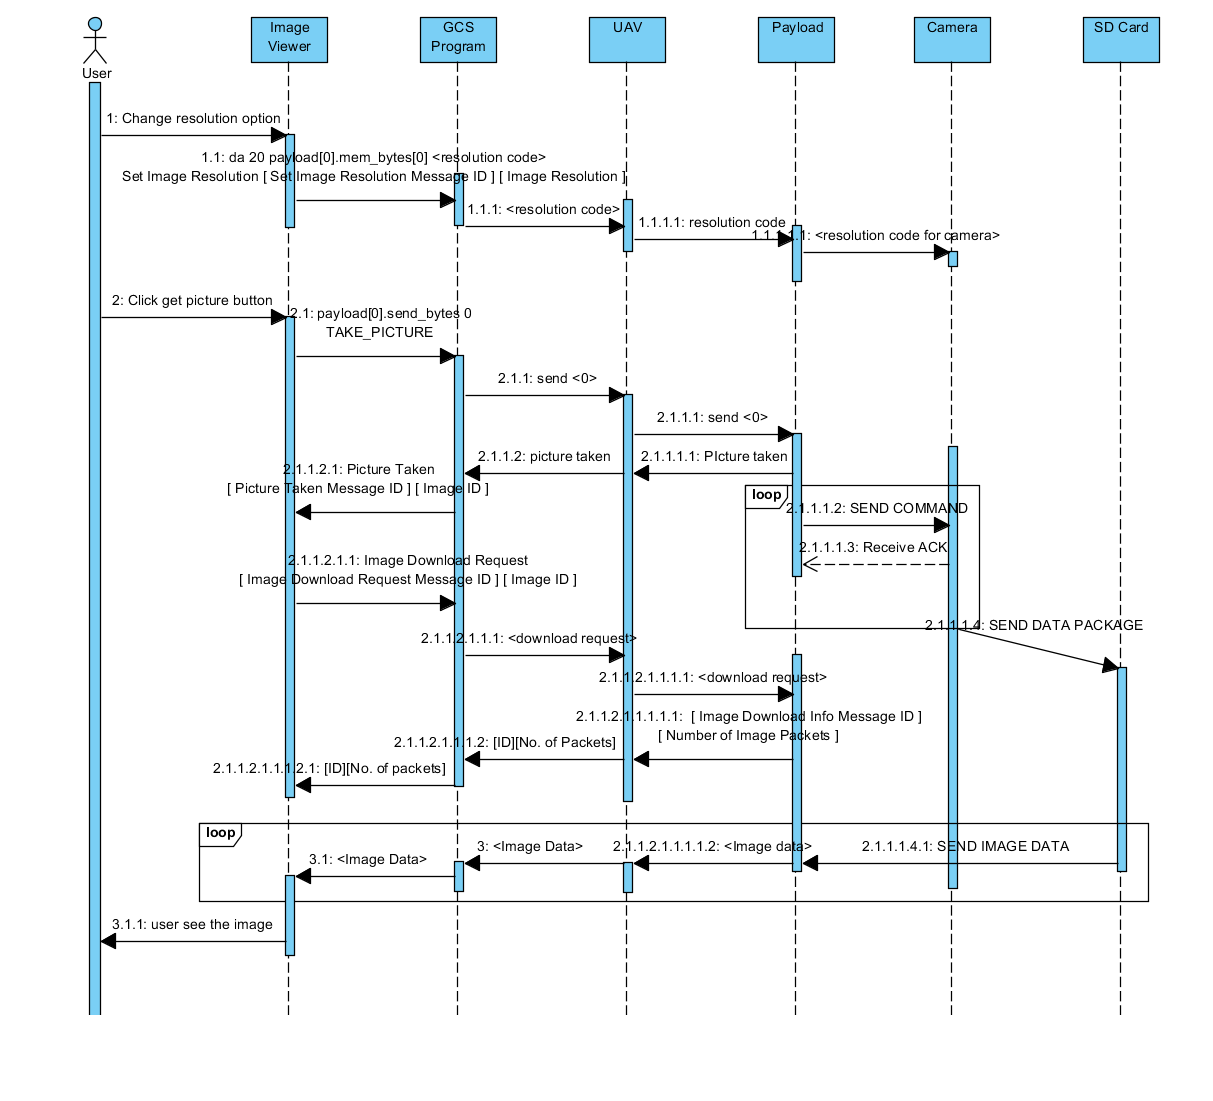
\includegraphics[width=1.00\textwidth]{figures/sequence_diagram.png} 
\end{center}
\caption{Sequence Diagram of the Data flow\label{sequence diagram}}
\end{figure}

Image data is also sent in the same basic manner, however the image is broken up into `packets' of data
which can be placed into the shared memory of the autopilot one at a time, as described by the \emph{Image Data}
message described above. One packet is sent for every transmit token sent by the autopilot, ensuring that the
payload module does not saturate the autopilot link with data. While packets are being sent, the main event loop
still checks for messages being sent from the ground station, allowing functionality such as the cancel download message 
to be implemented. In this way the payload module can transmit a whole image over the autopilot connection.

The testing of the image sending system is described in section \ref{sec:test_pl_image_send}, verifying the milestones 
as described.

Verification of milestone \ref{sec:ms_pl_img_gs_cam_res} (changing image resolution) can be seen in test \ref{sec:test_change_resolution}. Unfortunately changing colour type (milestone \ref{sec:ms_pl_img_gs_cam_colour_type})  was not fully implemented due to time constraints.

\subsection{Problems Encountered (mh)}
A number of problems were encountered and overcome during the implementation of the payload-ground station
communication code, a few of the most important are reproduced here.

\subsubsection*{Autopilot Bug (ab)}

The Autopilot sends "Transmit" tokens to the payload module every 20ms, 
to which a payload module sent an "ACK" token, even when it does not 
transmit any data. We encountered a problem whereby if our we tried to 
send any data to the payload during an "ACK", the autopilot would stop 
sending any "Transmit" tokens at all, effectively cutting off all 
communication to the payload module.

\begin{figure}[H]
  \centering
  \begin{tabular}{c c}
  \subfigure{\label{fig:testing_sc2_working1}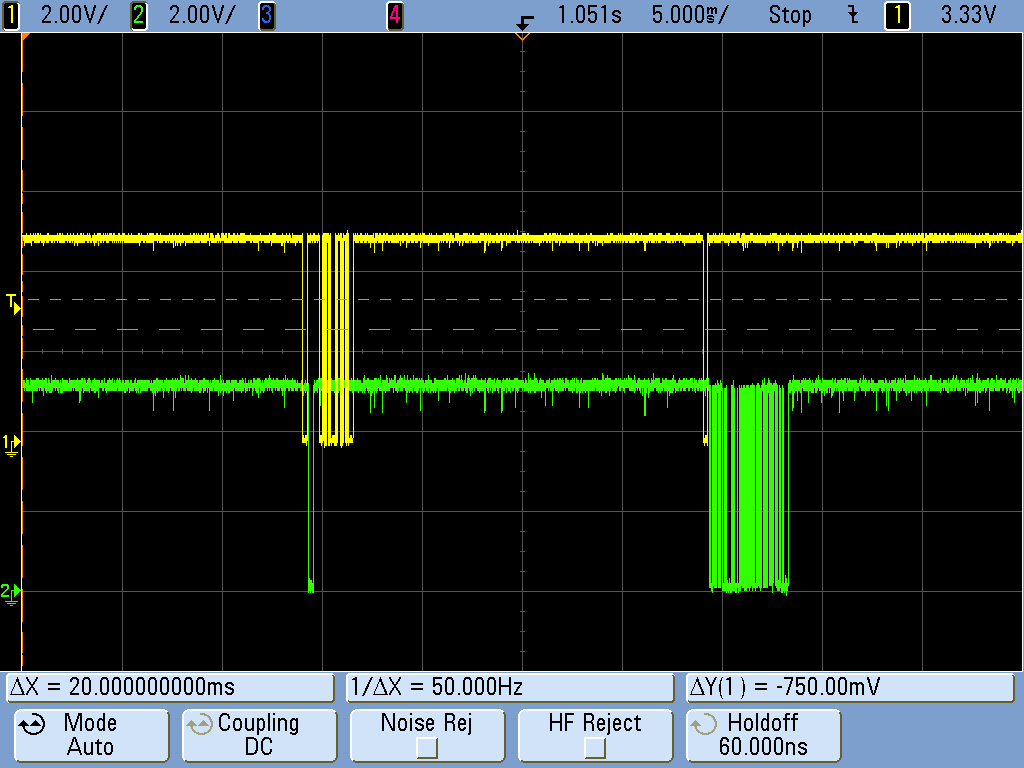
\includegraphics[width=0.5\textwidth]{scope/scope_1.png}}&                
  \subfigure{\label{fig:testing_sc2_working2}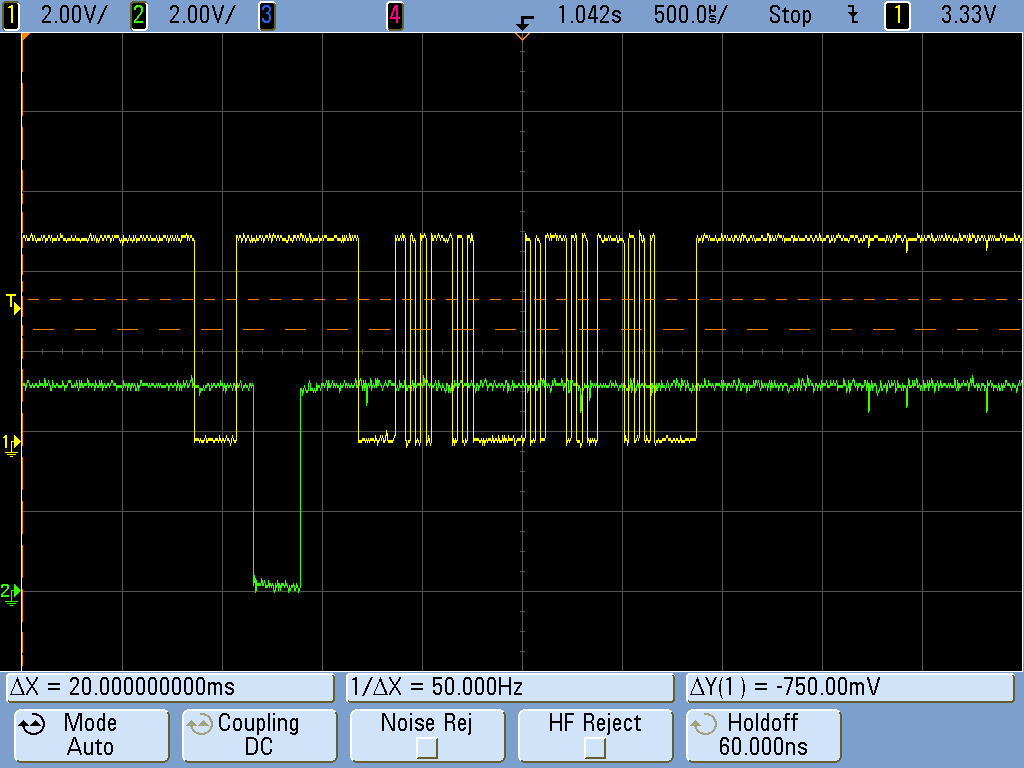
\includegraphics[width=0.5\textwidth]{scope/scope_2.png}} \\
  \subfigure{\label{fig:testing_sc2_working3}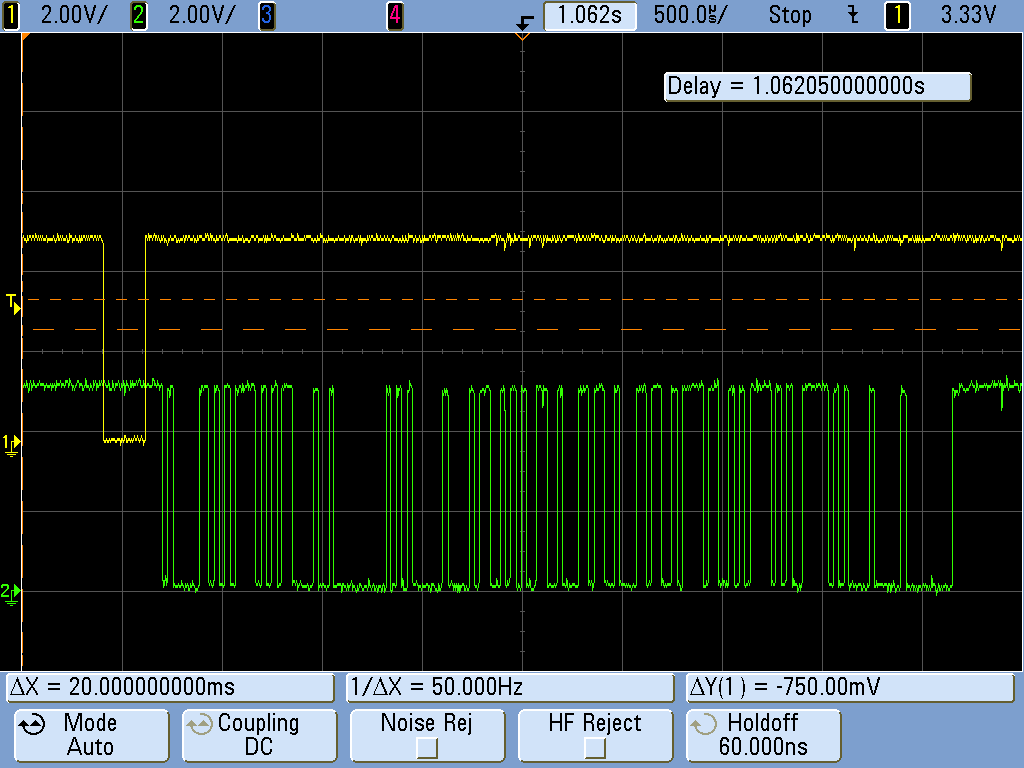
\includegraphics[width=0.5\textwidth]{scope/scope_3.png}}&                
  \subfigure{\label{fig:testing_sc2_working4}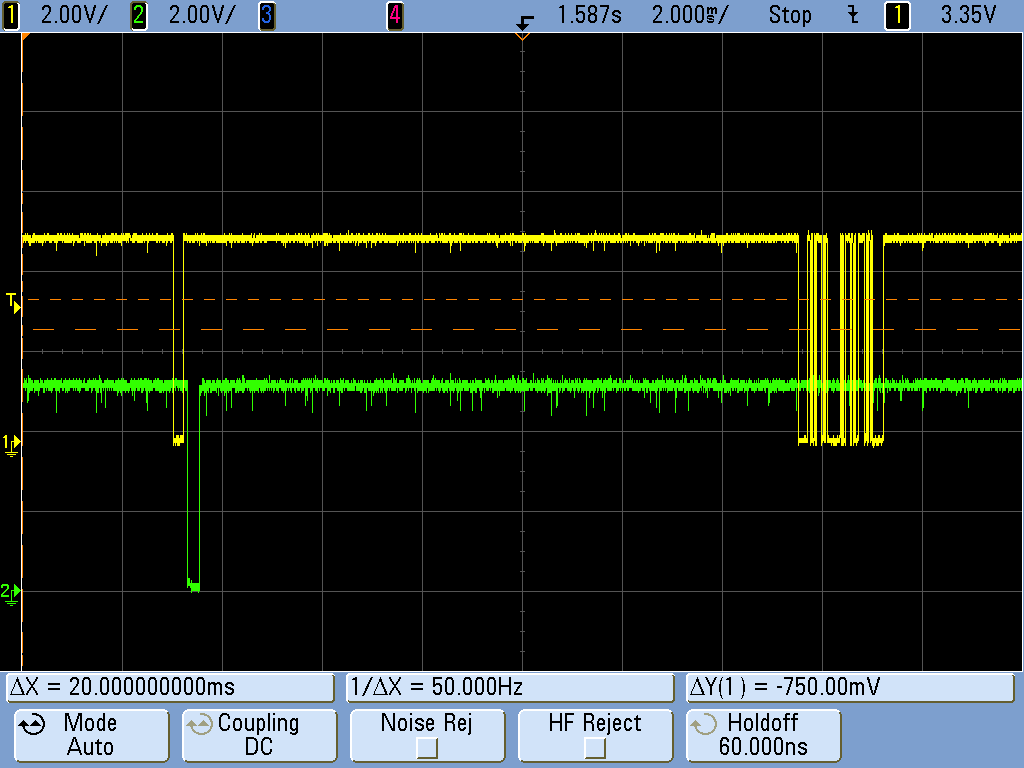
\includegraphics[width=0.5\textwidth]{scope/scope_11.png}}
  \end{tabular}
  \captionof{figure}{Oscilloscope traces for the situation where the autopilot does not break: In yellow is the Autopilot TX, in green the Payload TX. In this situation, after an ACK token is received by the autopilot, a SEND\_BYTES instruction is sent. On the next transmit token, a series of bytes is sent to the autopilot, and the autopilot continues to send Transmit tokens.}
  \label{fig:testing_sc2_working}
\end{figure}

\begin{figure}[H]
  \centering
  \begin{tabular}{c c}
  \subfigure{\label{fig:testing_sc2_broken1}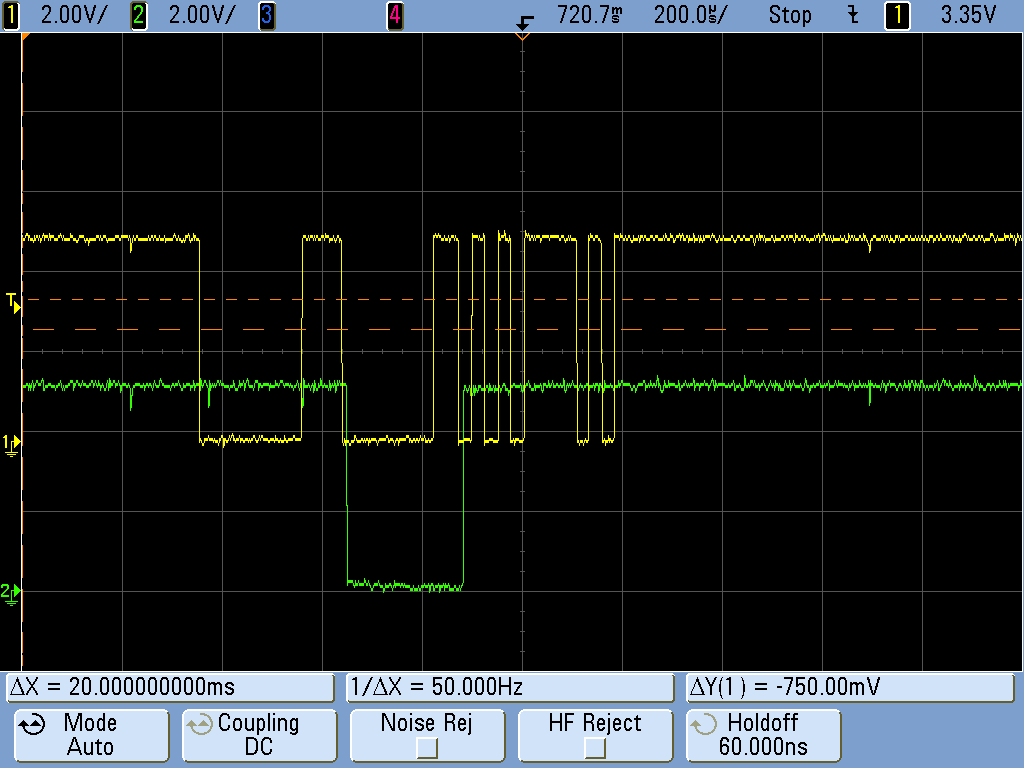
\includegraphics[width=0.5\textwidth]{scope/scope_6.png}}&                
  \subfigure{\label{fig:testing_sc2_broken2}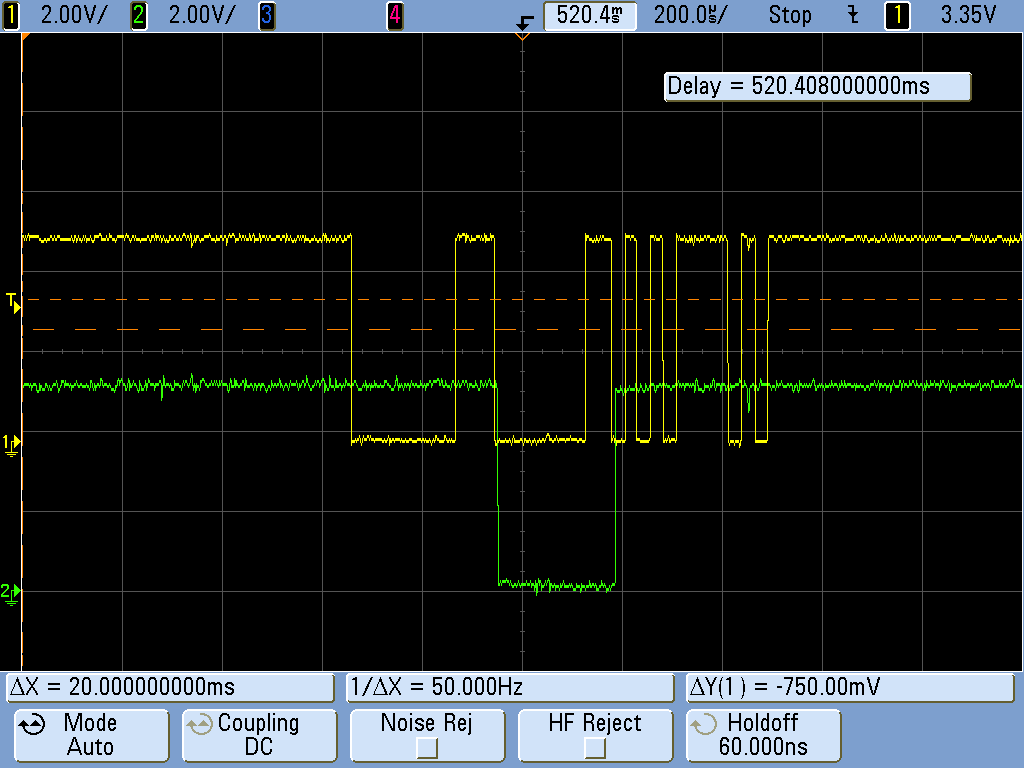
\includegraphics[width=0.5\textwidth]{scope/scope_14.png}} \\
  \subfigure{\label{fig:testing_sc2_broken3}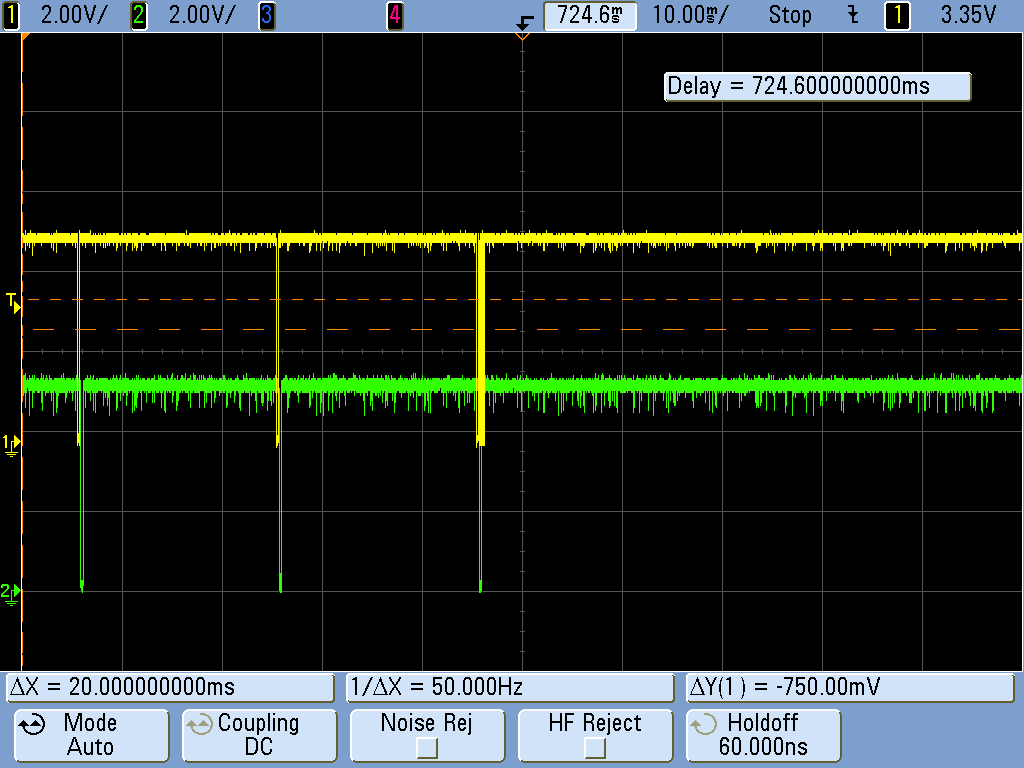
\includegraphics[width=0.5\textwidth]{scope/scope_7.png}}
  \end{tabular}
  \captionof{figure}{Oscilloscope traces for the situation where the autopilot breaks: In yellow is the Autopilot TX, in green the Payload TX. In this situation, whilst an ACK token is received by the autopilot, a SEND\_BYTES instruction is sent. No more transmit tokens are sent, therefore communication with the payload stops.}
  \label{fig:testing_sc2_broken}
\end{figure}

Not sure whether this was a bug with the Autopilot, we got in contact with 
our customer, sending all scope traces to him and a description of how 
to reproduce the error. Not being able to reproduce it with his dummy 
payload (strange, as our dummy payloads only differed in that his used a
surface-mount version of an ATmega168 and a MAX3070 transceiver instead 
of MAX489), he then came to ECS and debugged the Autopilot with us.

After a significant amount of time debugging the Autopilot and our 
payload, it was discovered this was indeed a problem with the Autopilot, 
which our customer was able to fix and subsequently update the firmware 
of our Autopilot.

\subsubsection*{Volatile Variables and ISRs (mh)}

Another problem encountered regarded a flag variable being checked in a function called in the main event loop. The flag
was the continuation condition of a while loop, and although it was being set in another section of code this new set 
value was not being propagated to the while loop code, meaning that the while loop would continue forever. This problem
was discovered (helped greatly by the debug interface described in section \ref{sec:payload_debug_interface}) . After some
consideration, research and experimentation it was discovered that the problem lay with the C compilers optimization. The 
flag was being set in a interrupt service routine (ISR), which the compiler assumed could not be called during the while loop
call, therefore it was optimized out, causing the loop to continue forever. The solution to this was to set this flag variable 
as \emph{volatile}, preventing it from being optimized out in this manner. The same was applied to all global variables modified in ISRs.


%|||||||| REMINDER: PROBLEMS CHALLENGES
%|||||||| REMINDER: HOW DID WE SOLVE PROBLEMS, DEBUGGING, TESTING, ETC
%|||||||| REMINDER: JOHN COULD TALK ABOUT HOW BROKEN CAMERAS SLOWED DOWN DEVELOPMENT BUT GOOD PLANNING AND CONTINGENCY MINIMISED RISK OR IN MANAGEMENT SECTION
%|||||||| REMINDER: FUTURE WORK
%|||||||| REMINDER: ADD NEWPAGES BETWEEN SECTIONS




\section{Ground Station Image Viewer}
The implementation of the program needs to start from many very basic programs such as connect to the port, change byte data to image, and change image to byte. 
So the first prototype was implemented by using console application in order to save time while debugging and we can see the output from the UAV. In order to see that the DataStream port stream data, the UAV set to send some data on the customer’s program, and then the data will be taken through the port and so we can see from the software.  

\subsection{Get Picture Function}
The 'Get Picture' functionality is the most important part of the GUI. The plan is when the user click on the Get Picture button, the program sends a string command to the ground station software with correct command bytes. Then the ground station software will generate a command byte and transmitted by TCP to the payload. Then the payload sends a ''Picture Taken'' command back through the data stream port. The GUI will then automatically send a download request command to the payload. The payload will then send image data back to the data stream port. The small programs that have been implemented in the early stage of development are reused here to send and receive data from the port. 

\subsection{File Dialogue}
For a .NET C\# Programming, there is a previous tools that we can use to change directory, open and save files. The OpenFileDialog,  SaveFileDialog, and FolderBrowser dialogue are existing classes that is suitable to do this job. However, to open any file dialogue, the application needs to have a STAThread in order to handle multiple objects. STAThread is an attribute which applied to the main method, indicating that the application should communicate with unmanaged COM code using the Single Threading Apartment. It allows main thread or the main form to run in the background while the file dialogue is executing. 

These file dialogues are not stated in the image viewer specification. But it has been implemented because the user may install the program in many computers and the initial folder might not exist and this might cause the system to give an error. It is also make the users feel that they can use the program more freely.  It also give the advantage of limiting the access to only an existing file, so there is no error when trying to save the image.

\subsubsection*{GUI connection}
 When the program start running, the program initialized the port and commands the customer’s application to tell the UAV to stream data to the data stream port. Figure~\ref{GCS_connect_command} shows the connection between the UAV data stream port and the ground station. The UAV has two ports, console port, and data stream port and it can send and receive any length of data. SEND\_ ZERO\_ TOKEN is designed by the customer’s so when the DataStream port receives this handshaking token, it will start streaming data. When any data transmission and receive, the software transfer the data through pipes. There are some global initializations that the software needs to perform only once when it is loaded for the first time. Note that the console port is manually connect by the ground control station software. The image viewer will give an error when there is no connection.
 The method to stream data is by writing this code to the user program:
 
\begin{center}
\texttt{da 20 ht}
\end{center}

''da'' defines which graph on the customer's program to display the data. ''20'' define the time period to send an amount of data in millisecond. ''ht'' is the customer's defined code to show height on da graph. 



\begin{figure}[!hbtp]
\begin{center}
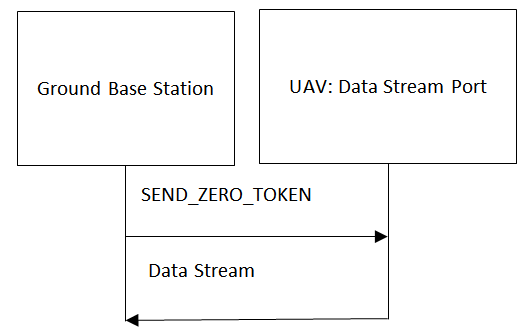
\includegraphics[scale=0.5]{figures/connect_command.png} 
\end{center}
\caption{The connection of data stream port\label{GCS_connect_command}}
\end{figure}


\subsubsection*{GUI data flow diagram}

\begin{figure}[!hbtp]
\begin{center}
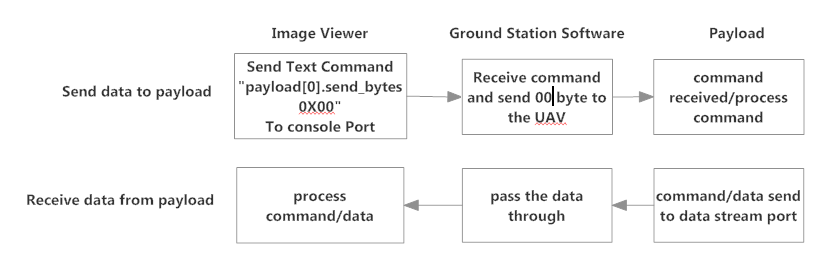
\includegraphics[scale=0.6]{figures/GCS_Payload_communication.PNG} 
\caption{The connection of data stream port\label{GCS_Payload_comm}}
\end{center}
\end{figure}

Table~\ref{command_table} shows how the command receive and send at ground station.SEND\_ZERO\_TOKEN is use for toggle the data stream port in order to make it send data to the image viewer. TAKE\_ PICTURE command sends 0 byte to command port by sending a string command to the UAV as shown in Figure~\ref{GCS_Payload_comm}. The PICTURE\_ TAKEN signal act in a similar way to ACK (acknowledgement) command which send back to the ground with a value of number of packet of the byte data. To ensure that the number of packet is the same in ground station and the UAV, the SEND\_ DOWNLOAD\_ REQUEST command sends back the information of number of packet. The number of packet shows how many cycle does the image view to do to receive all the data.  The payload will then send the DOWNLOAD\_ INFO to the ground station which follows by the IMAGE\_ DATA. The image data consist of 3 information bytes the first byte is always 4, this number tell the image view program that it is an image data. The next 2 bytes is saying which number of packet it is. If there is any packet skipped, the image viewer program will noticed and either send error or ask the UAV for the old set of packet. The image data at each cycle have a variable length. The program is designed to take the variable length of data.

\begin{table}[!htbp]

\begin{center}
\begin{tabular}{l l @{.} l}
 Command&
\multicolumn{2}{l}{Address Byte } \\

\hline
\underline{Command from Ground} & \\
SEND\_ZERO\_TOKEN & 0 \\
TAKE\_PICTURE & 0 \\
SEND\_DOWNLOAD\_REQUEST & 2 [MSB] [LSB]  \\
\\
\underline{Command received at Ground}\\
PICTURE\_TAKEN & 1 [MSB] [LSB]\\
DOWNLOAD\_INFO & 3 [MSB] [LSB]\\
IMAGE\_DATA & 4 $\overbrace{ [packet number]}^{2bytes} \overbrace{[image data]}^{data length}$ \\
\end{tabular}
\caption{Command table\label{command_table}}
\end{center}
\end{table}
 
 
\subsection{Code Highlight}

This section describe the code that is important for the program. The entire code will not be described but it will be in the appendix. In the image viewer program. It needs a class that can do these to port: connect, receive and send. FileStream class is a class in the .NET C\# which can create a file. BinaryWriter class used for writing the byte data into the generated file made by the FileStream class. The file directory will introduce a thread. While the open or save a file, the main application must be running, so the application need to deal with multi threads at the same time. Also when the get picture button got clicked, the main application is frozen because of the thread time organize do one thing at a time. The special code of thread need for handle this thread. 

\subsubsection*{Connect to UAV}
The Socket class has functions to send and receive byte and strings data. The handshaking protocol is using this code:

\begin{lstlisting}[caption={connect to port},label=lst:connectT]
public void ConnectToPort(Int32 portNumber, string portName)
{
        try            
        {
             Port.Connect(portName, portNumber);                
        }            
        catch 
        {            
            MessageBox.Show("Error code
                
             \n Unable to connect to dataStreamPort:
             \n Please check that:                
             \n1.The dataStreamPort is connected                 
             \n2.The program gcs has opened                 
             \n3.The program has connect to the dataStreamPort                
             \n4.The program has send stream data                
             \n5. The program as to run testbyte on da");                
        }            
}
        \end{lstlisting}

        
	The design of the .NET Socket class simply connect to a Port by a single command without any hesitation of changing the baud rate, stop bits, and parity bits. This advantage makes the Socket class a more useful class to work with the Port with existing and static set up. 

\subsubsection*{Start of the program}

\begin{lstlisting}[caption={Start of the program}, label=lst:payload_shared_mem_set]
	statusLabel.Text = ''Starting'';   
	progressBar.Value = 1;   
	string fileName = string.Format(''uavPictureAt { 0:yyyy-MM-dd_hh-mm-ss-tt}.jpg'', DateTime.Now);
	FileStream fileStream;
	fileStream = new FileStream(filePathTextBox.Text+''\\"+fileName, FileMode.Create);      
	BinaryWriter opFile = new BinaryWriter(fileStream);
	uavConn.SendTextToUAV("da 20 payload[0].mem_bytes[0]");      
 \end{lstlisting}
             In order to make the file name different and meaningful, the name of the picture will be the time and date of the time taken the picture. This has been done using the date and time class. fileStream was initiate to be in FileMode.Create, so it can create file. The BinaryWriter write the binary byte into a file in the directory of the fileStream. 
            
\texttt{string fileName = string.Format("uavPictureAt{ 0 : yyyy-MM-dd\_ hh-mm-ss-tt}
 .jpg", DateTime.Now);   }  
        
            This code time setting is valid for a file name. It will display year, month,date, and time in this order. The BinaryWriter class can create a binary file using specific data layout for its bytes. 

\subsubsection*{Change File Directory}
If the user wish to change the directory of the image taken, the image viewer program must support it. the mnuOpen\_click() method introduce an OpenFileDialog class. It begin with open file dialog box. This allow the user to open an inital image to the program. If the user took a picture, it will be saved in the same directory as the open file. This file dialog is limited to only the jpg picture in order to avoid the error of displaying the image. 
This file dialog introduce an extra thread. Without thread handler, the program will automatically organize the thread in the same timeline. This means it have to finish one event before it start another. The more detail about thread will be discussed in the thread section. 
\begin{lstlisting}[caption={change file directory},label=lst:changeFD]

        private void mnuOpen_Click(object sender, EventArgs e)        
        {        
             OpenFileDialog fileOpen = new OpenFileDialog();      
            
             fileOpen.Title = ''Select file to open:'';   
             fileOpen.Filter =''(* .JPG)| *.JPG; |(*.* )| *.* '';           

             if (fileOpen.ShowDialog() == DialogResult.OK)    
             {
    
                 updateDirectory(fileOpen.FileName);     
                 if (jpegList.Length != 0)     
                 {                    
                     pictureBox.Image = Image.FromFile(jpegList[filePathCount]);       
                 }         
                else       
                {       
                     pictureBox.Image = Image.FromFile(jpegList[0]);        
                }        
             }        
             pictureBox.SizeMode = PictureBoxSizeMode.StretchImage;       
             fileOpen.Dispose();        
        }       
        \end{lstlisting}
\subsubsection*{Threading}

A Scheduler that is reponsible for time-slicing threads controls the thread execution, manaing blocking of I/O message and signal handling\cite{keithC}. In any program there is always a main or initial thread running in a recursive loop that repond to the client application. In image viewer program, the main thread is the window application. When the get picture button got clicked, it will generate another less fundamental thread which will be execute after the loop have done. Therefore, in order to deal with this application while the picture is loading we need

\begin{center}
\texttt{Application.DoEvents();.}
\end{center}

During a process of taking picture and loading from the sky, the program wait for the loop to be finished before the user can do any action on the program. This is because while the code is processing, all other events wait in the queue, and it makes the program stop working. This can be fixed by using Application.DoEvents(). This code processes all of the Windows event messages that have queued up \cite{davidW}. When this code has been applied, the application can deal with other event at the same time as the code is running.


\begin{lstlisting}[caption={thread handling in the main},label=lst:threadH]
        [STAThread]        
        static void Main(string[] args)        
        {        
            mainForm.Show();
            while (true)            
            {            
                Application.DoEvents();                
            }
        	...
        \end{lstlisting}
        Application.DoEvents() in the Main function delegate that wraps the method that indicate where to start execution. The thread begin to run when the Application.DoEvents(); get called\cite{xieX}.When the file dialog try to run, the main application must be close. The [STAthread] has to be introduced in order to run multi thread at the same time. But, this doesn't mean the processor will be faster, but thread can make use of the resources that would go unused. A background thread can continue to run, while a foreground thread waits for the user input. This is called an apartment thread. 
        
\subsubsection*{Text Command}
TCP/IP protocols transfer data without modifying them. This allow the application to freely encode the data.\cite{davidB}.The Ground station software allow the program to send a stream of string in bytes and it will read the command bytes and send it to the payload on the UAV. The code has shown the way to implement the string and send a byte array to the payload.
	
	

\begin{lstlisting}[caption={send text in byte array},label=lst:sendT]
	 public void SendTextToUAV(string textToUAV)	        
         {        
             char[] toUAVChar = new char[512];       
             byte[] toUAVByte = new byte[512];        
             byte[] fromUAVByte = new byte[1000];       
             byte[] oneByteArray = new byte[1];       
             textToUAV += '' $\backslash$ n'';        
             toUAVChar = textToUAV.ToCharArray();        
             toUAVByte = System.Text.Encoding.ASCII.GetBytes(toUAVChar);       
             try       
             {      
                 int sendByte = consolePort.Send(toUAVByte, toUAVChar.Length, SocketFlags.None);     
             }     
            catch (SocketException ex)      
            {       
                Console.WriteLine(''ERROR\: '' + ex.Message);       
            }       
         }
\end{lstlisting}
                

To send text, the string of characters is translated into an array of bytes. American Standard Code for Information Interchange(ASCII) is use for translating English into a binary code. In the System.Text classes provide converting mechanism between each character sets. The ASCIIEncoding.GetBytes() is used for convert character array into a byte array.  
The Socket.Send() Method allow the user to send byte stream to the port connected.The customer's program will read from the port and display it onto the command line. The ''@ '' sign indicate that the command correctly sent from the application to the ground station software. The advantage of linking to the ground station software is that our customers can understand what is going on in the console line. For example:

\begin{center}
uavConn.SendTextToUAV(''da 20 payload[0].mem\_ bytes[0]'')\;
\end{center}

The text ''da 20 payload[0].mem\_ bytes[0]'' will be converted to char array and then to byte array. The byte array will then send the command to the console port to the payload by \texttt{consolePort.Send(toUAVByte, toUAVChar.Length)}. The customer is familiar with the ground station software program, so this method of sending data is satisfy. 

\subsubsection*{I/O Streams}
    The .NET framework's stream class is use as a powerful tools for encoding and decoding\cite{davidB}. In the image viewer program, we use FileStream to create a directory and to save the byte data into image. However, the program might have to deal with a corrupted image data. Framing is the problem of the receiver failed to find the beginning and the end of the message. The solution is the data packet give the information of how many loop must the program do in order to receive all the image data. The packet address locate in the second and third byte of the image data stream. 
     

\begin{lstlisting}[caption={writing binary file},label=lst:writingb]          
	for (int i = 3; i < packetSize; i++)
	{
          opFile.Write(packet[i]);
          numBytes++;
    	}
\end{lstlisting}         

       At every cycle of the data being received, opFile.Write() method will write the packet data into the file in the directory. After the cycle finished, the file will be saved and the image will be displayed in the picture box. 
\subsubsection*{Update the Directory}
The update directory method update itself every time the file directory is changing. This method will update the string of all the possible JPEG file in order to make it display in the picture box correctly. So when the left or right button got clocked, the string of JPEG file name will get plus or minus. This array of string have to update because it changes when the picture got deleted, or the new picture got taken. The array called \texttt{jpegList} is use as a string file storage for all the JPEG possible file
\begin{lstlisting}[caption=update directory class highlight, label=updateD]
            bool fileNameIsDirectory = false;
            if (fileName.Substring(fileName.Length - 4, 4).Contains("."))
            {
                fileDirectory = fileName.Substring(0, fileName.LastIndexOf("\\"));
                fileNameIsDirectory = false;

            }
            else
            {
                fileDirectory = fileName;
                fileNameIsDirectory = true;
            }
            filePathTextBox.Text = fileDirectory;
            try
            {
                jpegList = Directory.GetFiles(fileDirectory, "*.jpg");
            }
            catch
            {
            }
\end{lstlisting}
\subsubsection*{Other functions}
The user might want to delete some unwanted photo, so the delete button have been implemented. The delete button work like a normal file deleting button. But it has been complicated because the photo to delete must be the photo on the pictureBox. There is an error because the photo is using by the pictureBox. To fix this problem, the picture have to shifted left or right first and then delete the photo. This will solve almost all the problem. But where there is only one picture in the file, the program can not delete because even the pictureBox is set to null, it's last memory is still point at the deleting file. However, the disadvantage of the delete button is that if the wanted photo got deleted accidentally, it might take a long time to launch the UAV again and take the same photo.

\begin{figure}[!hbtp]
\begin{center}
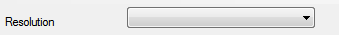
\includegraphics[scale=1]{figures/resolutionOption.PNG} 
\end{center}
\caption{The resolution in combo box\label{resolutionOption}}
\end{figure}
The camera has options of resolution as shown in Figure\ref{resolutionOption}. This can be useful when the speed is important. The lower the resolution, the faster the data transmitted to the ground. GUI has the combo box for the user to choose any wanted resolution in the options. The resolution allow user to have more accessible to the camera. However, this mean there is more on the programmer side to program the application.


The baud rate that we can transmit data from the UAV is 38.4kbaud. Bandwidth limitations severely restrict the volume of data to transfer over the wireless link. It takes around 8 to 20 seconds to transmit an image of resolution 640x480. This progress bar tells the user how much percentage of data received. The progress bar update at each cycle of the data receives. At the end of each image downloaded, the progress bar reset to its normal state.  The status text tells the user what signal have been sent or received. This status text ensures that the picture is downloading and it is good for testing that the tasking in process. These two nice application allocate on the bottom left of the GUI as shown in Figure\ref{progressBar}. However, these have to implement every cycle of the data collection and it might cause the cycle to run slower. The actual loop is much faster than the 38.4kbaud, therefore there is no problem implementing these in.
\begin{figure}[!hbtp]
\begin{center}
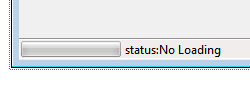
\includegraphics[scale=1]{figures/progressBar.PNG} 
\end{center}
\caption{The resolution in combo box\label{progressBar}}
\end{figure}


\subsection{Work Flow Diagram}
Describe Work Flow

\begin{figure}[!hbtp]
\begin{center}
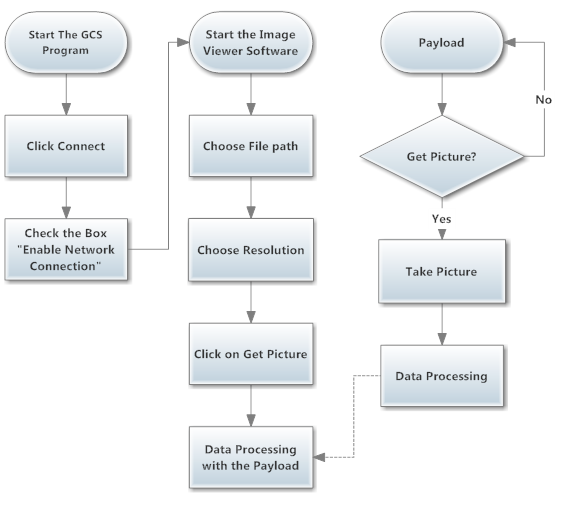
\includegraphics[scale=1]{figures/finalWorkFlow.PNG} 
\end{center}
\caption{Final work flow diagram of the GUI\label{GUI_finalWorkFlow}}
\end{figure}
\section{Progressive JPEG Manipulation}

\section{Physical Implementation}
\label{sec:PCB-implementation}

The final, delivered module is a $90mm\times62mm$ PCB. The PCB manufactured 
for the project was done so for free, using Spirit Circuits' "Go Naked"
service \cite{go-naked}. The PCB itself is a "tracks and holes" only service 
- no soldermask or silkscreen is applied. The schematic of the circuit 
delivered is available in Appendix ???, and of the PCB layout in Appendix 
???. A waterproof lacquer will be applied to the PCB to prevent condensation 
from shorting tracks together, and the module itself presented in a 
waterproof container before flight testing.

\begin{figure}[H]
        \centering
        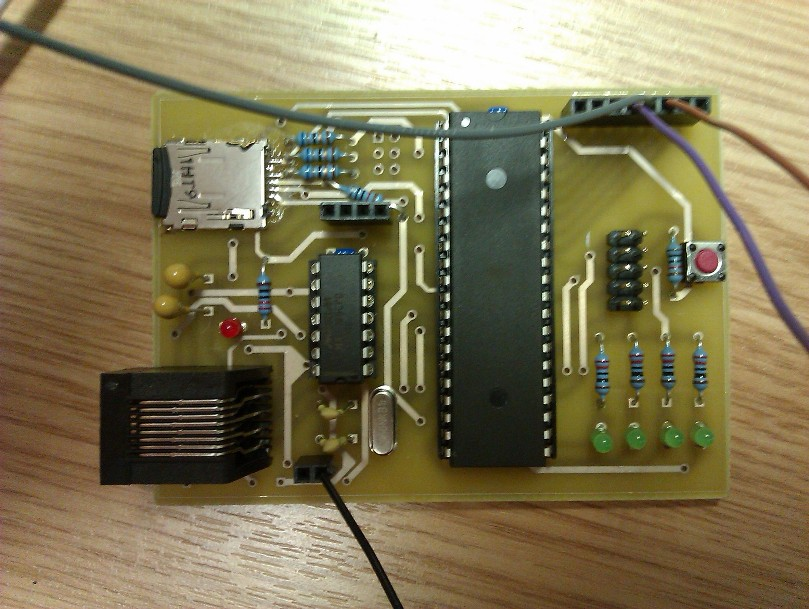
\includegraphics[width=1.00\textwidth]{figures/PayloadImplementation.jpg}
        \captionof{figure}{Image of the final payload, under test, before lacquer is applied. R11 can be seen between the Camera header and a via near the SD card Vcc}
        \label{fig:PayloadImplementation}
\end{figure}

Due to an issue discovered between ordering and receiving the PCB, an 
additional 10k$\Omega$ resistor has been placed between Camera RX and 3V3 (R11 
on the schematic). Also, the Single In Line header holes (for the Port A 
expansion and camera headers) have been widened from 0.40mm to 0.80mm. An 
update to the PCB layout is provided in the delivered repository.

The camera will also be presented in a sealed, weatherproof container.

\section{System Integration}

